% A good introduction to latex can be found here:
%    http://www.cse.ohio-state.edu/~hank/latex/lshort141.pdf

\documentclass[9.5pt]{extarticle}

\usepackage{full page}  % make the margins somewhat smaller than the default
\usepackage{graphicx}
\usepackage{amsmath}
\usepackage{indentfirst}
\usepackage{color}
\usepackage{cite}
\usepackage{wasysym}
\usepackage{amssymb}
\usepackage{multirow}
\usepackage{float}
\usepackage{lscape}
\usepackage{alltt} 
\usepackage{listings}
\usepackage{booktabs}
\usepackage{mathtools}
\usepackage{fancyhdr}
\usepackage[table,xcdraw]{xcolor}
\usepackage{hyperref}

\DeclarePairedDelimiter{\ceil}{\lceil}{\rceil}
\DeclarePairedDelimiter{\floor}{\lfloor}{\rfloor}

\definecolor{dkgreen}{rgb}{0,0.6,0}
\definecolor{gray}{rgb}{0.5,0.5,0.5}
\definecolor{mauve}{rgb}{0.58,0,0.82}


\usepackage{listings}  %  needed for source code listings

\lstset{frame=tb,
  language= java,
  aboveskip=1.5mm,
  belowskip=1.5mm,
  showstringspaces=false,
  columns=flexible,
  basicstyle={\small\ttfamily},
  keywordstyle=\color{blue},
  commentstyle=\color{dkgreen},
  stringstyle=\color{mauve},
  breaklines=true,
  tabsize=2,
  numbers=left,
  stepnumber=1,    
  firstnumber=1,
  numberfirstline=true
}
       

% set the document title, author, and date here.
%  once set, the \maketitle command (within the document)
%  will display them nicely
\title{A Simplified PageRank Method}
\author{Chua Zheng Fu Edrei}

\begin{document}
\maketitle

\section{Introduction}

In this report, I will present a simplified version of the PageRank method that Google uses to rank its webpages. I will discuss how we can use a Markov model to represent the link between webpages and construct a Markov transition matrix given a directed graph. We can solve for the stationary solution of the Markov chain problem by finding the eigenvector using the power method. I will also elaborate on how we can take into account dangling nodes and disconnected graph by using heuristic such as random surfing. The simplified version of PageRank will be implemented in Java and is tested on two simple network graphs (extracted from the Cornell Math Department webpage and the Wikipedia article on PageRank) to verify the correctness of the implementation. As an interesting experiment, I will also use the PageRank method on the Dartmouth Computer Science course dependency graph to rank computer science classes at Dartmouth. Finally, I will review an article by Kamvar et al (2003) on Extrapolation Method for Accelerating PageRank Computations and discuss how it is possible to compute an eigenvector in less time using Aitken and Quadratic extrapolation, which has important ramifications on ranking large databases.

\section{Basic Implementation}

\subsection{Problem statement}

The goal of the project is to implement a simplified version of the PageRank method used by Google to rank webpages in the internet. The basic idea is to consider the internet as a graph, with pages as vertices. We can have people uniformly distributed over vertices and conduct random walk in the graph by selecting random links. The PageRank algorithm seeks to address the question: in the limit, what is the stationary distribution of people over the pages. The more people there are on a certain page, the more important that page is. It is possible to construct this as a Markov model and eigen value problem. Because it is infeasible for me to test the simplified PageRank on the internet or on huge data network, I will attempt to demonstrate the utility of the method on the Dartmouth Computer Science course dependency graph and present some interesting results.

\subsection{Preprocessing}

My implementation takes in a text file (simple.txt, medium.txt, dartcsclass.txt etc.) as input. The format of the text file is straightforward. Each line of the text file contains two integers representing the ID of 2 different vertices separated by a white space, and the line can be interpreted as stating that there is an edge from the first vertex to the second vertex.\\

Most of the preprocessing of the text file take place in \verb`Graph.java`. The function \verb`createGraph` reads in the text file and convert it into a graph, which is represented using the data structure \verb`Map<Integer,Set<Integer>>`. The implementation of the function is given in Listing 1 and the basic idea is simple: loop through the entire text file and for each line, insert the first item and second item as vertices in the graph using \verb`checkVertices	` (if they are not already there) and add a directed edge between both vertices.\\

In addition, a \verb`Matrix` data structure is created to facilitate easy manipulation given that the PageRank method depends heavily on linear algebra concepts. Functions to support matrix manipulation (such as matrix multiplication with a vector or a constant) is given in \verb`Matrix.java` and the interested reader is encouraged to look at the source code for more details.

\begin{lstlisting}[language=java,caption={createGraph}]
	private void createGraph(String filename) {

        BufferedReader input = null;
        try {
            input = new BufferedReader(new FileReader(filename)); // Open file
            String pair;
            while ((pair = input.readLine()) != null) { // Read file and add int to map
                String[] parts = pair.split("\t");
                int first = Integer.parseInt(parts[0]);
                int second = Integer.parseInt(parts[1]);
                checkVertices(first,second);
                addEdge(first,second);

            }
        } catch (Exception e) {
            e.printStackTrace();
        } finally {
            // Close file if file exist. If not, catch the exception
            try {
                input.close();
            } catch (Exception e) {
                e.printStackTrace();
            }
        }
    }
\end{lstlisting}

\subsection{Constructing a Markov model}

\begin{figure}[H]
\centering
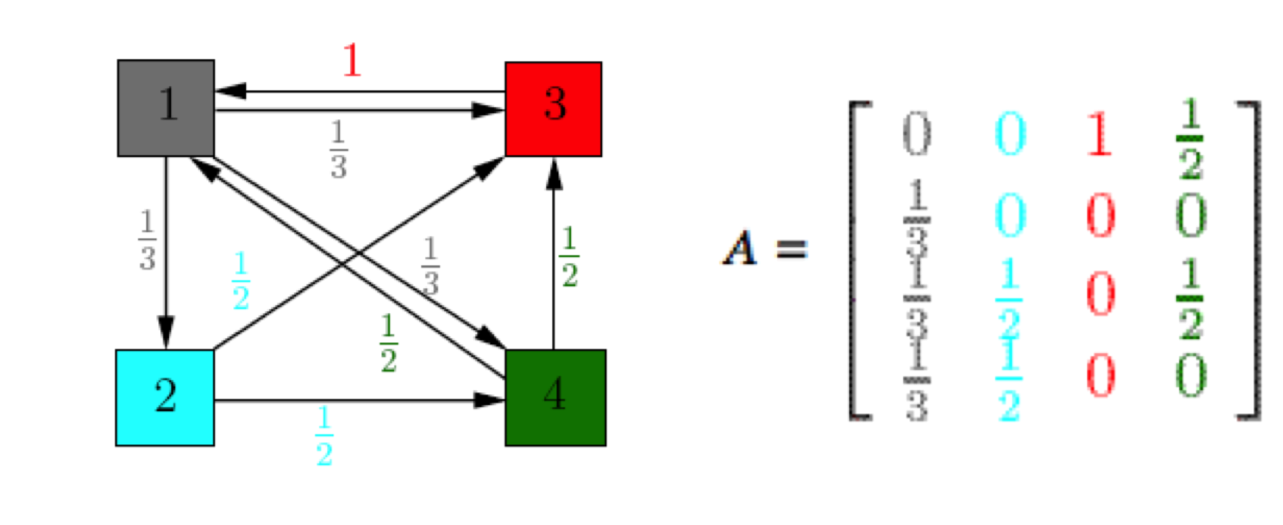
\includegraphics[scale=0.6]{page_rank_simple.png}
\caption{Construction of transition matrix for simple graph. Image source: Cornell Math Department Webpage}
\label{Figure 1}
\end{figure}

As mentioned in the introduction and the problem statement, the PageRank method uses a Markov model. Given the graph in Figure 1 for instance, we can construct a Markov transition matrix $A$. The entry $A_{ij}$ denotes the probability of a user randomly linking from page $i$ to page $j$. In the figure given, node 1 has 3 outgoing edges to node 2, 3 and 4 and a random surfer has a $\frac{1}{3}$ of going to any of the 3 vertices from node 1. Therefore $A_{10} = A_{20} = A_{30} = \frac{1}{3}$. Listing 2 gives the implementation for the \verb`constructTransition` function which constructs the transition matrix from the graph. The helper function \verb`numOutgoingEdges` counts the number of outgoing edges from a single vertex.


\begin{lstlisting}[language=java,caption={constructTransition}]
	private void constructTransition(Graph g){

        size = g.size();
        transition = new Matrix(size,size);
        index2value = new HashMap<>();

        int index = 0;
        for(int value : g.allVertices())
            index2value.put(index++,value);

        for(int c = 0; c < size; c++){
            for(int r = 0; r < size; r++){
                int first = index2value.get(c);
                int second = index2value.get(r);
                double p = g.numOutgoingEdges(first);

                if(g.hasEdge(first,second))
                    transition.data[r][c] = 1.0/p;
            }
        }
    }
\end{lstlisting}

\subsection{Power method}

In the Markov model, we have a transition matrix $A$ and a PageRank vector $\vec{v}$. At the beginning, all the entries in $\vec{v}$ will be $1/n$, where $n$ is the number of pages or vertices, since we assume that users are uniformly distributed across all webpages. This leads to a Markov chain problem: in the limit, we are interested in the distribution of people over pages i.e. $\vec{v_n} = A^n\vec{v_0}$ as $n \to \infty$. $v_n[i]$ will give us the probability of landing at page $i$ given a random walk over time, which give us a measure of how important the page is. 

\begin{lstlisting}[language=java,caption={powerMethod}]
    public double[] powerMethod(double[] vect, double epsilon, int max_k){

        int k = 1;
        double delta = Double.MAX_VALUE;
        double[] prevVect = vect;

        while(delta > epsilon && k < max_k){
            double[] newVect = multiplyVector(prevVect);
            delta = distance(newVect, prevVect);
            prevVect = newVect;
            k++;
        }
        return prevVect;
    }
\end{lstlisting}

We recognize the search for a stationary distribution as an eigenvector problem, which is a well-researched problem in linear algebra. The solution can be obtained using a power method, which is given in Listing 3. The basic idea is to compute the vector multiplication of $A$ with $\vec{v}$ repeatedly until the vector $\vec{v}$ converges. A parameter $\epsilon$, measures the convergence of the vector by calculating the eucildean distance between $\vec{v_n}$ and $\vec{v_{n-1}}$. The code for calculating the euclidean distance is straightforward and is presented in Listing 4.


\begin{lstlisting}[language=java,caption={distance}]
    private double distance(double[] v1, double[] v2){

        double sum = 0;
        for(int i = 0; i < v1.length; i++){
            sum += Math.pow(v1[i] - v2[i],2);
        }
        return Math.sqrt(sum);
    }
\end{lstlisting}

\section{Additional Considerations}

We have constructed the ranking problem as a Markov model and have also presented the solution as an eigenvector problem that can be solved using the power method. In this sense, the model is complete. However, in real graphs, there are often additional considerations involved that might complicate things and lead to the formulation of a problem in which there is either no eigenvector solution (the problem does not converge) or a solution that is trivial (all zeros). To circumvent this problem, we consider heuristic for dangling nodes or link and disconnected graph.

\subsection{Dangling nodes}

\begin{figure}[H]
\centering
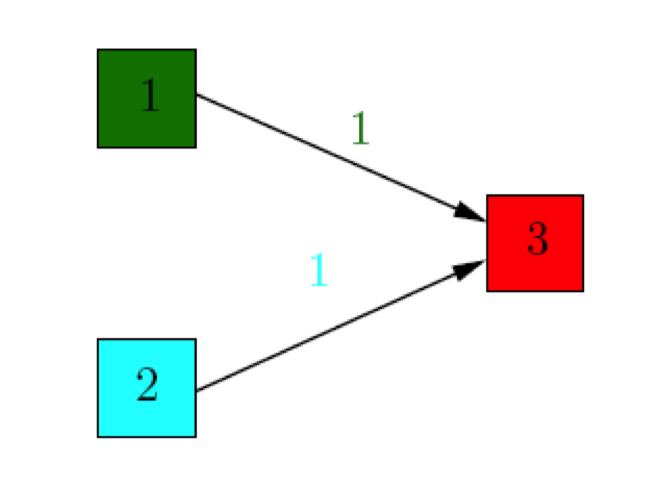
\includegraphics[scale=0.5]{dangling.png}
\caption{Example of dangling nodes. Image Source: Cornell Math Department Webpage}
\label{Figure 2}
\end{figure}

Figure 2 shows a graph in which a vertex (node 3) does not have any outgoing edges. Node 3 is referred to as a dangling node. In the matrix formulation of the problem, the eigenvector is noted to be a zero vector (trivial solution). However, this is counterintuitive and it is obvious that node 3 should have some importance since it has incoming links. \\

An easy fix to this problem is suggested by Page et al, and it involves replacing the column that is represented by node 3 with a column vector with all the entries as $\frac{1}{3}$. This will allow the importance of node 3 to be equally distributed across all the vertices instead of being lost. The implementation of this improvement is given in Listing 5, and the basic idea is to replace all zero columns with a column vector of entries $1/n$.

\begin{lstlisting}[language=java,caption={enforceDanglingNodes}]
	private void enforceDanglingNodes(){

        for(int c = 0; c < size; c++){
            if(!hasOutgoingEdge(c)){
                fillColumn(c, 1.0/(double)size);
            }
        }
    }
\end{lstlisting}

\subsection{Disconnected graphs}

\begin{figure}[H]
\centering
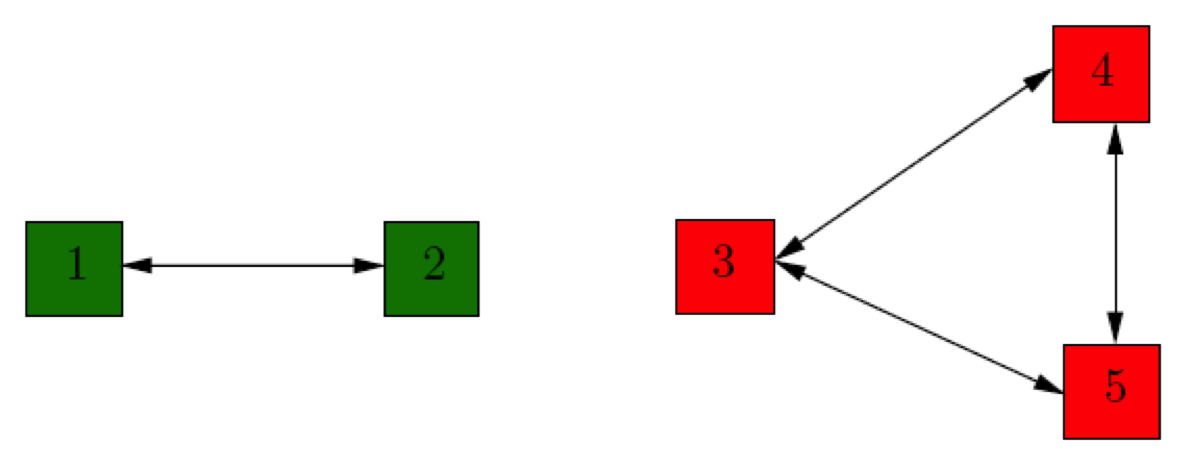
\includegraphics[scale=0.5]{disconnected.png}
\caption{Example of disconnected graph. Image Source: Cornell Math Department Webpage}
\label{Figure 3}
\end{figure}

Disconnected graph is annother problem that might occur in ranking web pages. Figure 3 shows a disconnected graph in which a random surfer that starts in the green portion of the graph will never be able to get to the red portion of the graph. Page et al noted that disconnected graphs will yield multiple eigenvector solution that are often not linear combination of each other so that in theory, the notation of ranking pages from the first connected component relative to the ones from the second connected component is ambiguous. \\

Page et al suggested that in order to fix the problem, we can introduce a damping factor $p$ that is $0<p<1$ (the value used by Google is $p = 0.15$). We can define the PageRank matrix $M = (1-p)\dot A + p\dot B$, where $A$ is the transition matrix and $B$ is a matrix of the same dimension as $A$ and with all entries as $1/n$. $M$ can be proved to be a column stochastic matrix with only positive entries and by the Perron-Frobenius Theorem, it implies that the eigenvalue problem will have an eigenvalue of multiplicity one, which is what we want. \\

This resolution also make intuitive sense: $M$ suggests that most of the time, the random surfer will follow an outgoing link and move to a neighbouring vertex. But there is a small probability $p$ that the surfer might quit the current page and ``jump'' or ``teleport'' to a new one randomly.\\

Listing 6 gives the implementation for \verb`randomJump` that takes into account the random jumping or teleporting that might happen as described above.

\begin{lstlisting}[language=java,caption={randomJump}]
    private void randomJump(double damping){

        Matrix B = new Matrix(size,size);

        for(int r = 0; r < size; r++)
            Arrays.fill(B.data[r],1);

        B.multiplyConstant(damping/(double)size);
        transition.multiplyConstant(1-damping);
        transition.addMatrix(B);

    }
\end{lstlisting}

\section{Results and Discussion}

To check the validity and correctness of my code, I checked my output against the worked solution to a Homework problem assigned by the Cornell Math Department. The input is the graph that is given in Figure 1 (simple.txt). The solution given in the homework problem is $[0.38,0.12,0.29,0.19]$ for nodes 1, 2, 3 and 4 respectively. The output from my code (in sorted order of rank) is given in Listing 7 and 8. We can see that the values agree, suggesting that my approach is giving the correct result.\\

Listing 7 shows the output for PageRank on the simple graph without jumping, while Listing 8 shows the output with the jumping heuristic. It can be noted that the output generated by the PageRank method with the jumping or teleporting heuristic results in higher ranked pages received a lower ranking and lower ranked pages receiving a higher ranking. This makes intuitive sense, since we account for the possibility that a random surfer might leave a page that is higher ranked and teleport to a page with lower ranking.\\

\begin{lstlisting}[language=java,caption={Output for PageRank on simple graph without jumping}]
Results sorted in decreasing order of rank or importance

1 = 38.7110%
3 = 29.0328%
4 = 19.3544%
2 = 12.9018%

\end{lstlisting}

\begin{lstlisting}[language=java,caption={Output for PageRank on simple graph with jumping}]
Results sorted in decreasing order of rank or importance

1 = 36.8150%
3 = 28.7969%
4 = 20.2081%
2 = 14.1801%

\end{lstlisting}
~\\

To further verify the correctness of my code, I checked my output against a more complicated graph that is presented in the Wikipedia article for PageRank. The graph is given in Figure 4. The caption to the Figure in Wikipedia noted that the PageRank values are obtained using a random jump heuristic with a damping factor of $p = 0.15$. Using the same parameter value, I run the code and obtain the output in Listing 9. Again, I noted that my results agree with the expected result, boosting my confidence in the correctness of my approach.\\

It is also interesting to note that Page C has a higher PageRank than Page E, even though there are fewer links to C. This is because the one link to Page C comes from an important page that has a lot more links (Page A) and thus a random surfer has a higher likelihood of reaching Page C compared to E. This demonstrates the underlying principle behind the PageRank algorithm.\\

\begin{figure}[H]
\centering
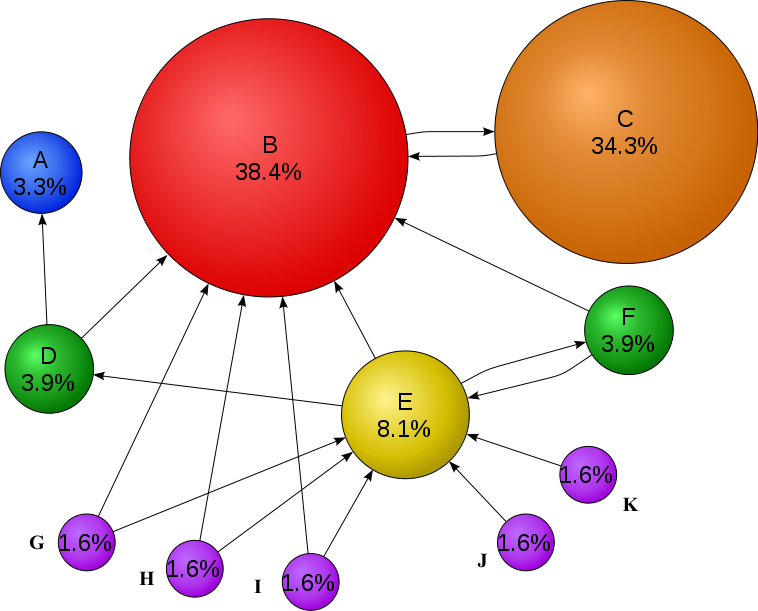
\includegraphics[scale=0.35]{page_rank_wiki.png}
\caption{Experiment with a simple network with page rank calculated using dangling nodes correction and random link jump with damping factor 0.15. Image source: Wikipedia PageRank article}
\label{Figure 4}
\end{figure}

\begin{lstlisting}[language=java,caption={Output for PageRank on medium graph with jumping}]
Results sorted in decreasing order of rank or importance

2 = 38.4370%	// B
3 = 34.2941%	// C
5 = 8.0886%	 	// E
4 = 3.9087%		// D
6 = 3.9087%		// F
1 = 3.2781%		// A
7 = 1.6169%		// G
8 = 1.6169%		// H
9 = 1.6169%		// I
10 = 1.6169%	// J
11 = 1.6169%	// K

\end{lstlisting}
~\\

As an interesting side project, I decided to use the simplified PageRank algorithm that I have developed on the Dartmouth Computer Science course dependency graph given in Figure 5. I made a significant adjustment in my text file: I reverse all the edges i.e. I convert all incoming edges in Figure 5 to outgoing edges and vice versa. This is because it is more helpful to define a dependency relationship between course $i$ and $j$ as one where a person who have taken a course $i$ must have taken a course $j$ in the past (having taken $i$ implies that the person have taken $j$, another way to see it is the material covered in course $i$ reference the material in course $j$). In addition, we note in Figure 5 that one of the classes is labelled LA, which I will replace with a course number of 100. \\

I am interested to investigate which computer science course at Dartmouth is the most important class using the PageRank algorithm by that definition. The results for the top 12 (just so that we can include CS76, which is ranked 12th, in the ranking) ranked classes is given in Listing 10. The full Listing can be found in the Appendix. Unsurprisingly, CS 1, CS 10, CS 50, CS 31 and CS 51 dominates the ranking. There is a high probability that a random student that is surfing the CS department course dependency graph will find himself ending up in CS 1, CS 10, CS 50, CS 31 and CS 51 about $50\%$ of the time, or in our representation, it means a student taking a CS class is more likely to refer back to material taught in the above 5 classes than any other classes! 

\begin{figure}[H]
\centering
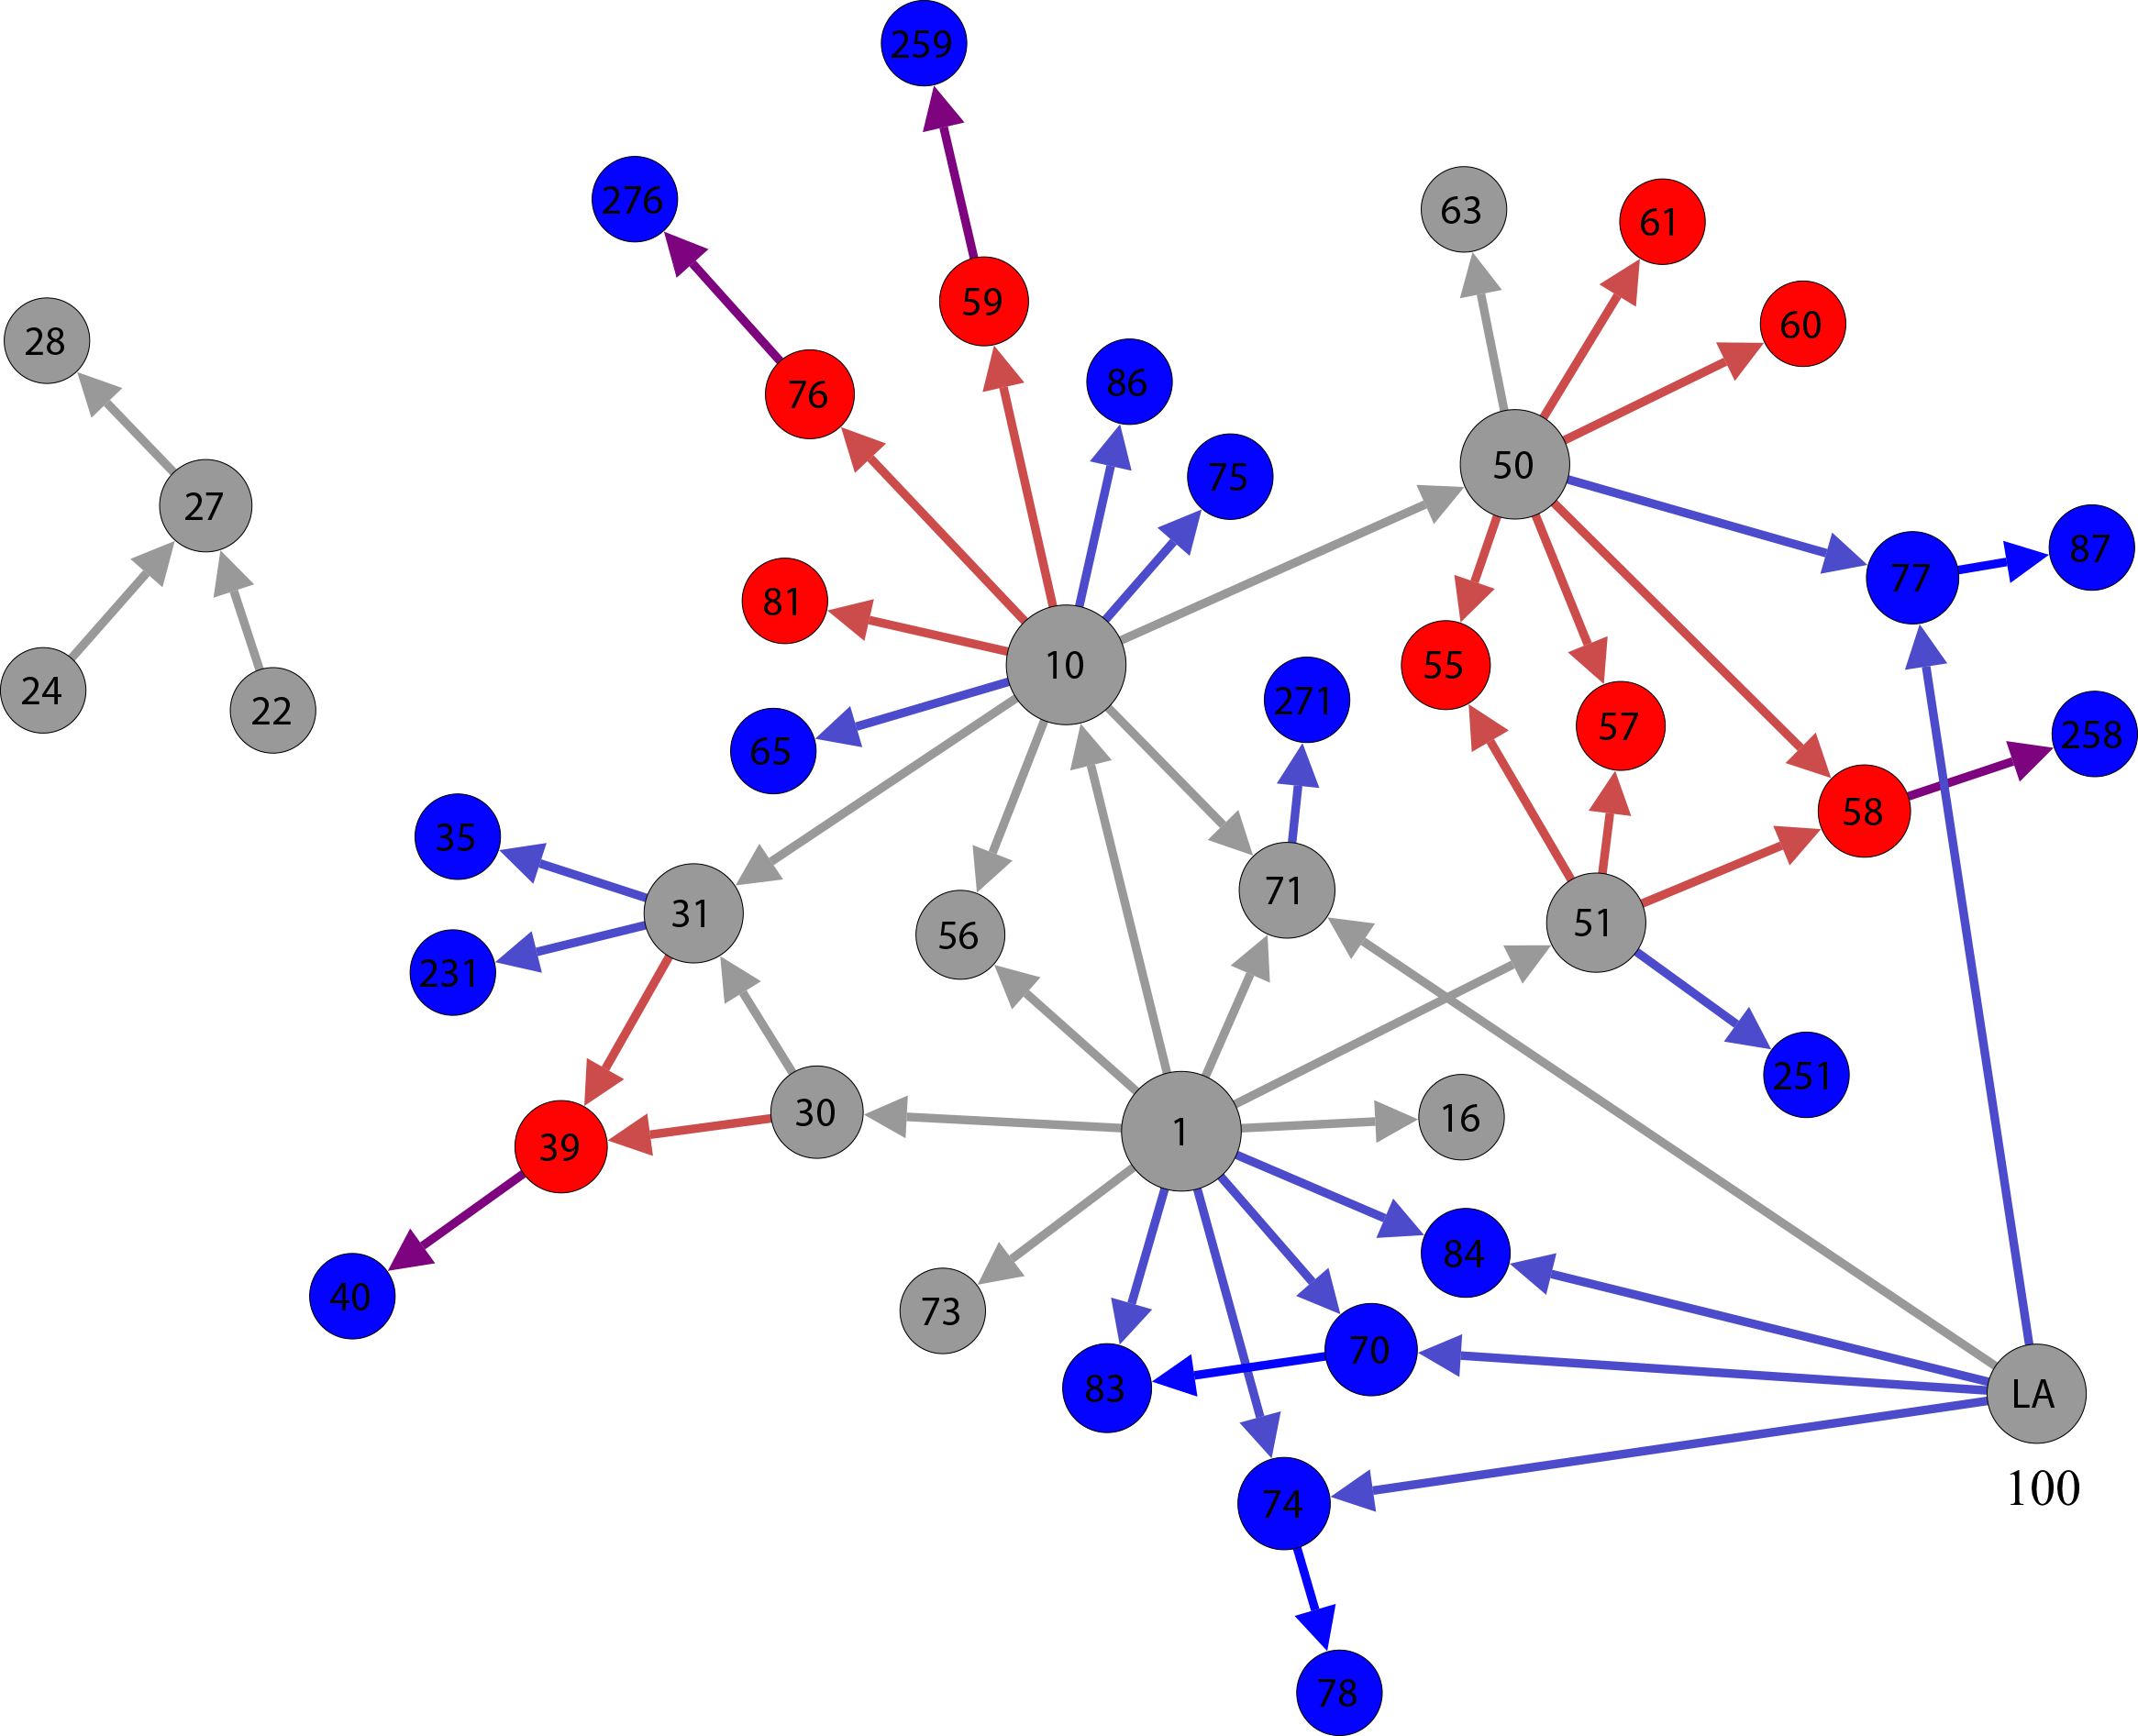
\includegraphics[scale=0.17]{course_dependencies.png}
\caption{Experiment with the Dartmouth Computer Science Course Dependency graph. Image source: Dartmouth Computer Science Department page}
\label{Figure 5}
\end{figure}

\begin{lstlisting}[language=java,caption={Truncated Output for PageRank on Course Dependency Graph (Full result is in Appendix)}]
Results sorted in decreasing order of rank or importance

1 = 23.3493%
10 = 14.3853%
50 = 5.7083%
100 = 3.9446%
31 = 3.3322%
51 = 3.3322%
30 = 3.1233%
58 = 1.7684%
71 = 1.7684%
74 = 1.7684%
59 = 1.7684%
76 = 1.7684%

\end{lstlisting}


\section{Literature Review}

I reviewed the aarticle by Kamvar S., Haveliwala T., Manning C., Golub G on Extrapolation Methods for Accelerating PageRank Computations (Kamvar et al, 2003). In this article, Kamvar et al pointed out correctly that the biggest bottleneck in the PageRank algorithm is the computation of the eigenvector (or finding the solution for $\vec{v_n} = A^n\vec{v_0}$ as $n \to \infty$. The traditional method is the power method, which is computationally expensive and the runtime is not ideal. Inverting the transition matrix to find the eigenvector is not computationally feasible either because it is difficult to invert a large matrix (the web is a huge network of pages).\\

The authors proposed two different method of computing an eigenvector that is proven to have superior runtime time compared to the power method, and they refer to it as the Aitken extrapolation method and the Quadratic extrapolation method. The algorithms are derived using polynomial division and the Cayley-Hamilton Theorem. The basic idea is that by keeping track of additional coefficients and vectors (that can be solved using linear algebra techniques such as Gram-Schmidt), we are able to improve the runtime of the algorithm.\\

The extrapolation methods increase the convergence rate and the amount of computational time required. As an added bonus, they are fairly simple to implement and requires little additional infrastructure to integrate into the standard power method.\\

I find this article interesting because I noted how a computer science is closely related to Mathematics and how the use of Mathematical formalism and tools is often useful in coming up with new algorithms.



\section{Conclusion}


In this report, I have implemented a simplified version of PageRank and explored in further depth the topic of Markov chain and eigenvalue problem in computer science. In addition, I have also investigated additional improvement by considering dangling links and random teleportation from one page to another. I have tested my code on the Dartmouth Computer Science course dependency graph, and obtain some interesting results. \\

I have also included in the source code directory a text file ``physcitation.txt'' that shows the relationship between citations by authors in the field of General Relativity and Quantum Physics as I am personally interested as a Physics major in knowing which physicists is ranked more highly using the PageRank algorithm. The data is collected from the ArxiV and Stanford Large Network Dataset collection. I have ran the code and generated results, however I am unable to find a mapping between the numerical ID in the text file given in the dataset with the actual name of the Physicists (let me know if you manage to find the mapping online!).\\
 
Possible extension to the project includes implementing sparse matrix storage and improving the runtime of  solving for the eigenvector by considering other methods such as Aitken or Quadratic extrapolation. It will also be interesting to see the results of the PageRank method on a social network such as LinkedIn or Facebook.

\newpage

\section{References}

Cornell Math Department. Lecture \#3: PageRank Algorithm - The Mathematics of Google Search. Accessed on 2 March 2016. Retrieved from \url{http://www.math.cornell.edu/~mec/Winter2009/RalucaRemus/Lecture3/lecture3.html}\\

Dartmouth Computer Science Course Dependency Graph. Accessed on 2 March 2016. Retrieved from \url{https://web.cs.dartmouth.edu/sites/cs.dartmouth.edu/files/course_dependencies.png}\\

Kamvar S., Haveliwala T., Manning C., Golub G.. Extrapolation Methods for Accelerating PageRank
Computations, WWW '03 Proceedings of the 12th international conference on World Wide Web: 261 - 270, 2003.\\

Page, Lawrence, Brin, Sergey, Motwani, Rajeev, Winograd, Terry. The PageRank Citation Ranking: Bringing Order to the Web. Technical Report. Stanford InfoLab. 1999.\\

Rousseau C. How Google works: Markov chains and eigenvalues. Accessed on 2 March 2016. Retrieved from \url{http://blog.kleinproject.org/?p=280}\\

Wikipedia. PageRank article. Accessed on 2 March 2016. Retrieved from \url{https://en.wikipedia.org/wiki/PageRank#Simplified_algorithm}\\

\newpage
\section{Appendix}

\begin{lstlisting}[language=java,caption={Output for PageRank on Course Dependency Graph}]
Results sorted in decreasing order of rank or importance

1 = 23.3493%
10 = 14.3853%
50 = 5.7083%
100 = 3.9446%
31 = 3.3322%
51 = 3.3322%
30 = 3.1233%
58 = 1.7684%
71 = 1.7684%
74 = 1.7684%
59 = 1.7684%
76 = 1.7684%
39 = 1.7684%
77 = 1.7684%
27 = 1.7684%
22 = 1.7074%
24 = 1.7074%
70 = 1.3622%
65 = 0.9560%
258 = 0.9560%
259 = 0.9560%
73 = 0.9560%
75 = 0.9560%
78 = 0.9560%
271 = 0.9560%
16 = 0.9560%
81 = 0.9560%
83 = 0.9560%
84 = 0.9560%
276 = 0.9560%
86 = 0.9560%
87 = 0.9560%
28 = 0.9560%
35 = 0.9560%
231 = 0.9560%
40 = 0.9560%
55 = 0.9560%
56 = 0.9560%
57 = 0.9560%
251 = 0.9560%
60 = 0.9560%
61 = 0.9560%
63 = 0.9560%
\end{lstlisting}


\end{document}